\subsubsection{A 200 Reference BPM Map}
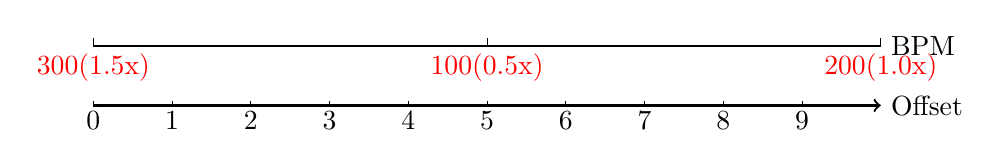
\begin{tikzpicture}

\draw [thick] (0,0) -- (10,0) node [anchor=west] {BPM};
\draw [thick, ->] (0,-0.75) -- (10,-0.75) node [anchor=west] {Offset};
\foreach \x in {0,1,2,3,4,5,6,7,8,9}
    \draw (\x cm,-0.75) -- (\x cm,-0.70) node[anchor=north] {$\x$};

\draw (0.0,0.0)  -- (0.0,0.1)  node [anchor=north,yshift=-0.7mm]{\textcolor{red}{300(1.5x)}};
\draw (5.0,0.0)  -- (5.0,0.1)  node [anchor=north,yshift=-0.7mm]{\textcolor{red}{100(0.5x)}};
\draw (10.0,0.0) -- (10.0,0.1) node [anchor=north,yshift=-0.7mm]{\textcolor{red}{200(1.0x)}};

\end{tikzpicture}

\begin{table}[h!]
  \begin{center}
    \label{tab:norm_t1}
    \begin{tabular}{c|r|l}
      \textbf{Offset} & \textbf{BPM} & \textbf{$Scroll_{BPM}$}\\
      \hline
      0  & 300 & 1.5x\\
      5  & 100 & 0.5x\\
      10 & 200 & -\\
      
    \end{tabular}
  \end{center}
\end{table}